\documentclass[13pt, t]{beamer}

% Presento style file
\usepackage{config/presento}

% custom command and packages
% custom packages
\usepackage{textpos}
\setlength{\TPHorizModule}{1cm}
\setlength{\TPVertModule}{1cm}

\newcommand\crule[1][black]{\textcolor{#1}{\rule{2cm}{2cm}}}



\usebackgroundtemplate{
\includegraphics[height=\paperheight]{images/background.jpg}}

\title{\Large lingtypology: R пакет для лингвистического картографирования}
\author[shortname]{\large Г. Мороз}
\institute[shortinst]{\large Лаборатория языковой конвергенции, НИУ ВШЭ}
\date{\large 
\begin{center} 
18 декабря 2018 г. \bigskip \\ 
{\color{colorblue} Открытые лекции — «Городские данные»\\ 
Софт Культуры и Инфокультуры} \bigskip \bigskip  \bigskip \\
ссылка на презентацию: \href{https://tinyurl.com/ycx46od6}{tinyurl.com/ycx46od6}
\end{center}
}

\begin{document}

% Title page
\begin{frame}[plain]
\maketitle
\end{frame}

\framecard[colorblue]{{\color{colorblue} \huge \#тыжлингвист}}

\begin{frame}{\#тыжлингвист}
\begin{itemize}
\item  умеет читать на всех письменностях мира
\item знает все языки на свете
\item умеет распознавать каждый язык на слух \pause
\item может рассказать о происхождении каждого слова \pause
\item пишет без ошибок и знает все правила орфографии \pause
\item не знает математики и программирования \pause
\end{itemize}
\Large все вышеперечисленное, конечно, неправда
\end{frame}

\begin{frame}{Лингвистика}
\begin{itemize}
\item прескриптивная \pause
\item вся остальная
\begin{itemize}
\item исследования грамматики языка и языкового разнообразия
\item исследования распределения грамматических особенностей в языках мира
\item исследования когнитивных способностей человека и других животных, связанных с языком
\item исследования в области NLP и их приложения
\item исследования в области синтеза и распознования речи и языка
\item создание компьютерных инструментов для решения самых разных задач
\end{itemize}
\end{itemize}
\vfill
Еще бывает \textit{компьютерная лингвистика}:
\begin{itemize}
\item вспомогательные инструменты лингвистического исследования и документации
\item Computational linguistics
\item NLP
\end{itemize}
\end{frame}

\framecard[colorblue]{{\color{colorblue} \huge лингвистические базы данных}}

\begin{frame}{Лингвистические базы данных}
\alert{\large Корпуса --- базы данных языкового материала}
\begin{itemize}
\item корпус литературных текстов
\item \href{http://ruscorpora.ru/}{Русский национальный корпус}
\item аудио и видео корпуса \pause
\begin{itemize}
\item настоящая речь, а не тексты
\item см., например, \href{http://www.parasolcorpus.org/Pushkino/login.php}{Корпус бассейна реки Устья}
\item см., например, \href{http://www.parasolcorpus.org/Rogovatka/}{Корпус села Роговатка}
\item см., например, \href{http://rsl.nstu.ru}{корпус русского жестового языка}
\item см., например, \href{https://www.youtube.com/watch?v=OUwOvF7TqgA&feature=youtu.be&t=1m25s}{Уошо}
\end{itemize}
\end{itemize}
\vfill
\alert{\large Базы данных языковых структуру}
\begin{itemize}
\item \href{https://wals.info/}{The World Atlas of Language Structures (WALS)}
\item \href{https://ewave-atlas.org/}{World Atlas of Varieties of English (eWAVE)}
\item \href{https://glottolog.org/}{Glottolog} --- система ссылок на языки мира.
\item ... \href{https://clld.org/datasets.html}{и другие}
\end{itemize}
\end{frame}

\begin{frame}{\href{https://glottolog.org/}{Glottolog}}
\alert{\large Адыгейский язык назван в литературе:}
\begin{itemize}
\item \textit{черкесскiй} или \textit{адигскiй} --- [Люлье 1846]
\item \textit{адыгейский язык} --- [Рогава, Керашева 1966]
\item \textit{West Circassian} --- [Smeets 1984]
\item \textit{Tcherkesse occidental} --- [Paris, Batouka 2005]
\item \textit{Adyghe} --- [Korotkova, Lander 2010]
\item еще встречается \textit{нижнечеркесский}, \textit{западночеркесский}, \textit{западноадыгский}, \textit{кяхский} \pause
\end{itemize}
\vfill
\alert{\large На все это есть один код: \href{https://glottolog.org/resource/languoid/id/adyg1241}{\texttt{adyg1241}}}
\end{frame}

\begin{frame}{\href{https://ropensci.github.io/lingtypology/}{lingtypology}}
\alert{\large Glottolog + Leaflet}\\
\vfill
\texttt{\small map.feature(c("Adyghe"{}, "Russian"{}, "Polish"))}\\
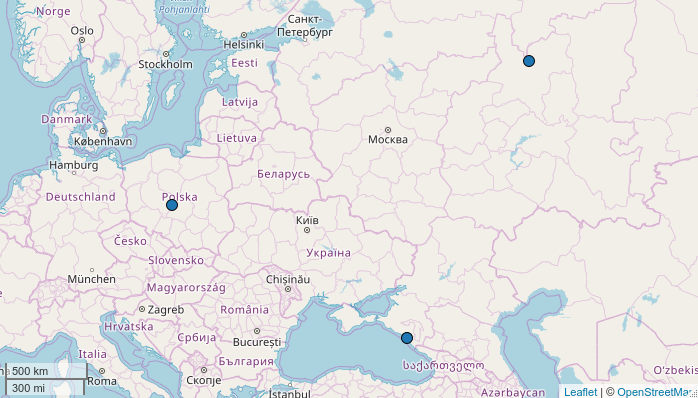
\includegraphics[width=\linewidth]{images/01-map}
\end{frame}

\begin{frame}{\href{https://ropensci.github.io/lingtypology/}{lingtypology}}
\alert{\large Glottolog + Leaflet}\\
\vfill
\texttt{\small map.feature(lang.aff("Sign"))}\\
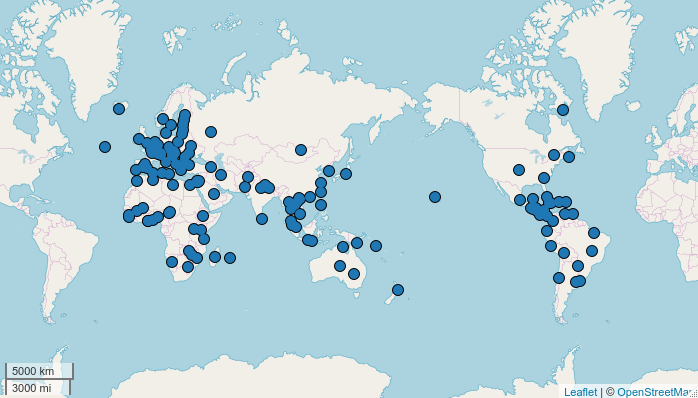
\includegraphics[width=\linewidth]{images/02-sign}
\end{frame}

\begin{frame}{\href{https://ropensci.github.io/lingtypology/}{lingtypology}}
\alert{\large Glottolog + Leaflet}\\
\vfill
\texttt{\small  map.feature(c(lang.aff("Slavic"), lang.aff("Celtic")),}\\
\texttt{\small \ \ \ \ \ \ \ \ \ \ \ \ c(rep("Slavic"{}, 20), rep("Celtic"{}, 6)))}\\
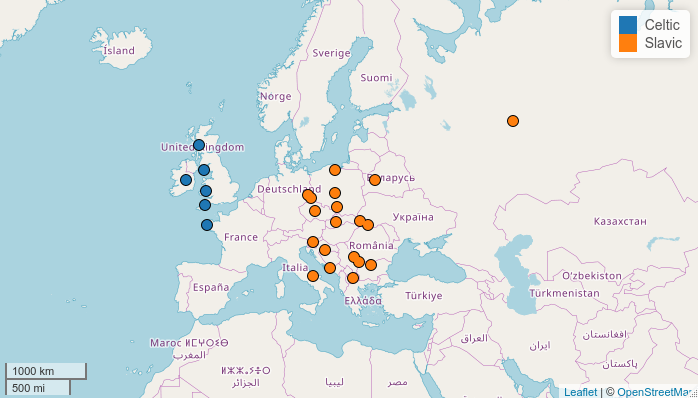
\includegraphics[width=\linewidth]{images/03-colored}
\end{frame}

\begin{frame}{\href{https://ropensci.github.io/lingtypology/}{lingtypology}}
\alert{\large Glottolog + Leaflet}\\
\vfill
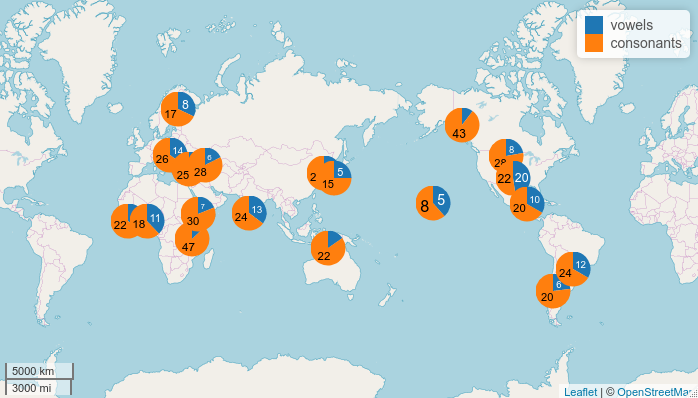
\includegraphics[width=\linewidth]{images/04-minicharts}
\end{frame}

\begin{frame}{\href{https://ropensci.github.io/lingtypology/}{lingtypology}}
\alert{\large Glottolog + Leaflet}\\
\vfill
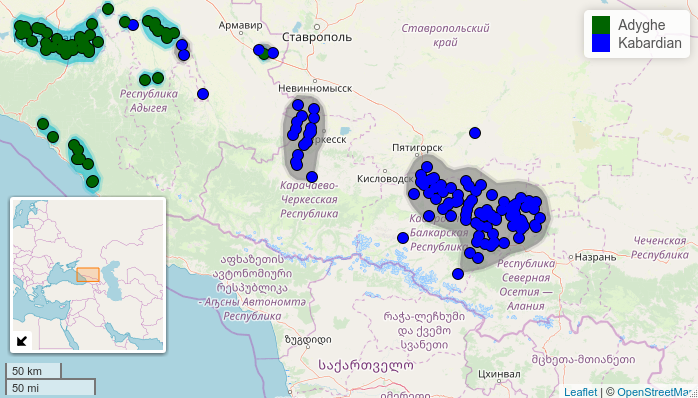
\includegraphics[width=\linewidth]{images/05-density}
\end{frame}

\begin{frame}{\href{https://ropensci.github.io/lingtypology/}{lingtypology}}
\alert{\large Glottolog + Leaflet}\\
\vfill
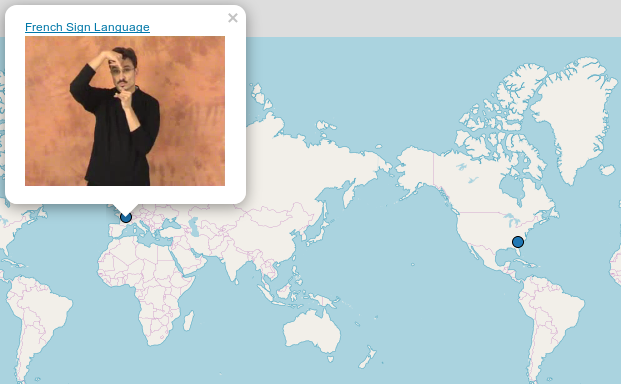
\includegraphics[width=\linewidth]{images/06-sign}
\end{frame}

\begin{frame}{Результаты:}
\begin{itemize}
\item Более 14 тыс. скачиваний \pause
\item В lingtypology внедрились API для других лингвистических баз данных\pause
\item Множество редакций туториала; лекции и мастерклассы\pause
\item Появляются базы данных, основанные на lingtypology:
\begin{itemize}
\item \href{https://agricolamz.github.io/wwsd/}{The World Writing System Database  (WWSD)}
\item \href{https://agricolamz.github.io/wcad/}{The World Consonant Alternation Database}
\item \href{https://daghestanian-sound-database.herokuapp.com/}{Daghestanian Sound Database}
\item \href{https://agricolamz.github.io/The_Circassian_Isoglosses_Database/}{The Circassian Isoglosses Database}
\item \href{https://agricolamz.github.io/uvular_database/}{Uvular consonants in Languages of the Caucasus}
\item \href{https://sl-iconicity.shinyapps.io/iconicity_patterns/}{Iconicity patterns in Sign Languges}
\item \href{https://agricolamz.github.io/scsd/}{The Sound Change in Sibilants Database}
\item Typological atlas of Guatemala \pause
\end{itemize}
\item 6 issues на \href{https://github.com/clld/glottolog}{гитхабе Glottolog'а} \pause
\item \href{https://github.com/ropensci/software-review/issues/95}{рецензия rOpenSci} \pause
\item все больше появляется студенческих работ с картами
\end{itemize}
\end{frame}

\framecard[colorblue]{{\color{colorblue} \huge Спасибо за внимание! \bigskip\\
\Large Пишите письма\\
agricolamz@gmail.com\bigskip\\
Рисуйте карты с \href{https://ropensci.github.io/lingtypology/}{lingtypology}
}}

\end{document}